\documentclass[10pt]{beamer}

\usetheme{default}

\usepackage[utf8]{inputenc}
\usepackage[russian]{babel}
\usepackage[OT1]{fontenc}
\usepackage{amsmath}
\usepackage{amsfonts}
\usepackage{amssymb}
\usepackage{graphicx}
\usepackage{etoolbox}
\usepackage{caption}
\usepackage{subcaption}
\captionsetup{compatibility=false}
\usepackage{booktabs}
\usepackage{array}



\makeatletter



\setbeamercolor{title}{fg=white}
\setbeamercolor{frametitle}{fg=black}
\setbeamerfont*{title}{family=\sffamily,size=\LARGE}

\setbeamerfont{page number in head/foot}{size=\scriptsize}
\setbeamertemplate{footline}[frame number]
\let\otp\titlepage
\renewcommand{\titlepage}{\otp\addtocounter{framenumber}{-1}}

\setbeamertemplate{background canvas}{%
	\ifnumequal{\c@framenumber}{0}{%
      
\includegraphics[width=\paperwidth,height=\paperheight]{images/cover.png}
   }{%
      \ifnumequal{\c@framenumber}{\inserttotalframenumber}{
         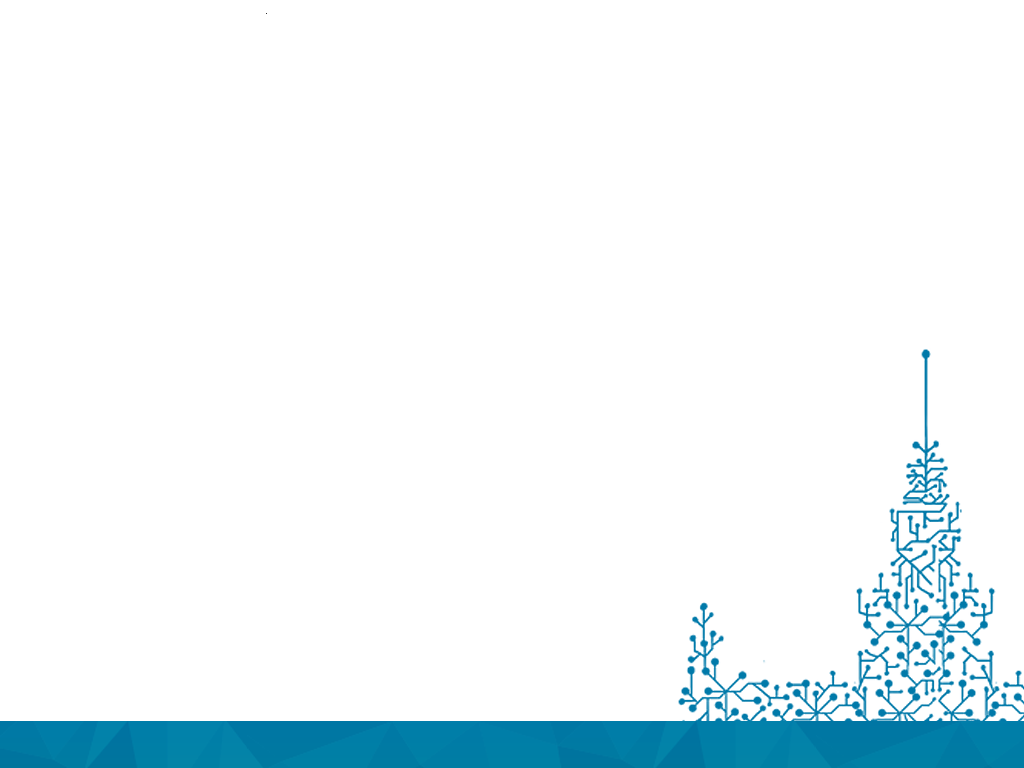
\includegraphics[width=\paperwidth,height=\paperheight]{images/back.png}
      }{%
         % Other frames
      }%
   }%
}

\makeatother

\beamertemplatenavigationsymbolsempty

\author{Нестеров Павел}
\title{\newline \newline \newline Лекция n2 \\ Softmax слой \\ Ограниченная машина Больцмана}

\begin{document}

\begin{frame}[plain]
\titlepage
\end{frame}

\begin{frame}{План лекции}
\tableofcontents
\end{frame}


\section{Вспоминаем прошлую лекцию}

\begin{frame}{Модифицированная модель нейрона МакКаллока-Питтса}

\begin{figure}[h!]
  \centering
  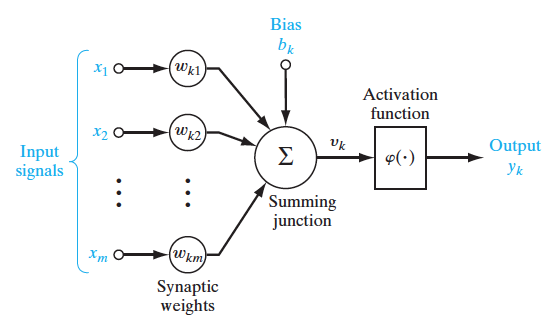
\includegraphics[width=1\textwidth]{images/neuron_mod.png}
  \caption{Схема искусственного нейрона\footnote{Neural Networks and Learning Machines (3rd Edition), Simon O. Haykin}}
\end{figure}

\end{frame}

\begin{frame}{Многоснойная нейронная сеть прямого распространения}

\begin{figure}[h!]
  \centering
  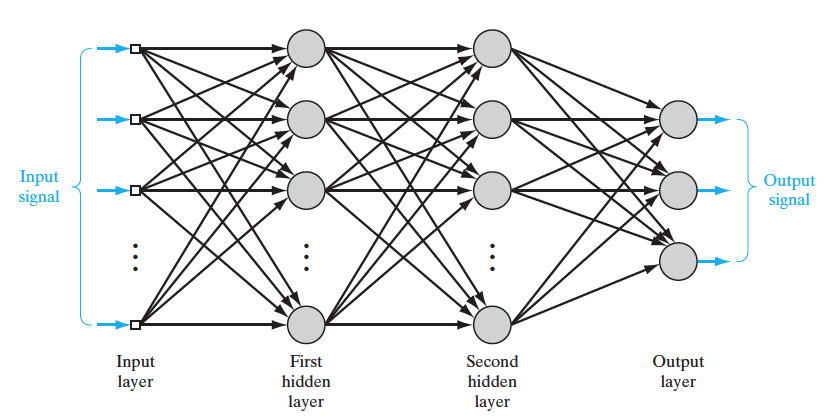
\includegraphics[width=1\textwidth]{images/mlp.png}
  \caption{Архитектура сети с двумя скрытыми слоями\footnote{Neural Networks and Learning Machines (3rd Edition), Simon O. Haykin}}
\end{figure}

\end{frame}

\begin{frame}{Алгоритм обратного распространения ошибки}

\begin{figure}[h!]
  \centering
  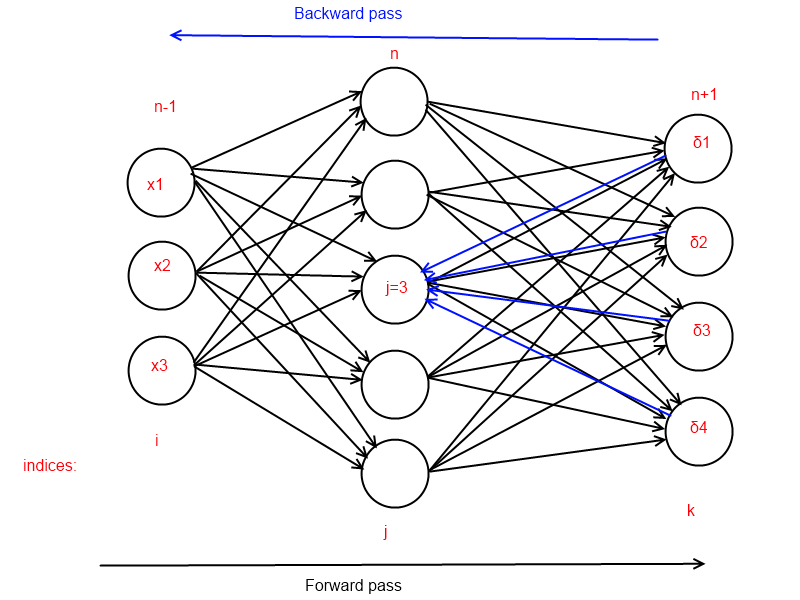
\includegraphics[width=0.9\textwidth]{images/f_b_pass.png}
  \caption{Схема прямого (нелинейного) и обратного (линейного) распространения сигнала в сети}
\end{figure}

\end{frame}


\begin{frame}{Некоторые функции стоимости}

Среднеквадратичная ошибка:
\begin{itemize}
	\item $E = \dfrac{1}{2} \sum_{i \in \textsc{output}} \left( t_i - y_i \right)^2$
	\item $\dfrac{\partial E}{\partial y_i} = y_i - t_i$
\end{itemize}

Логарифм правдоподобия Бернулли: 
\begin{itemize}
	\item $E = -\sum_{i \in \textsc{output}} \left( t_i \log y_i + \left( 1 - t_i \right) \log\left( 1 - y_i \right) \right)$
	\item $\dfrac{\partial E}{\partial y_i} = \dfrac{t_i}{y_i} - \dfrac{1 - t_i}{1 - y_i}$
\end{itemize}

\textit{Для каких задач машинного обучения удобны эти функции?}

\end{frame}


\section{Softmax слой}

\begin{frame}{Вспоминаем логистическую регрессию, два класса}

\begin{itemize}
	\item $D = \left\{ \left( x_i, y_i \right) \right\}_{i=1\ldots m}, \forall x_i \in \mathbb{R}^n, \forall y_i \in \left\{ 0, 1 \right\}$
\end{itemize}
\begin{eqnarray*}
P(y = 1, x) &=& \frac{P(x | y)\cdot P(y)}{P(x | y)\cdot P(y) + P(x | \overline{y})\cdot P(\overline{y})} \\
&=& \frac{1}{1 + \exp\left( \frac{P(x | y)\cdot P(y)}{P(x | \overline{y})\cdot P(\overline{y})} \right)} \\
&=& \frac{1}{1 + e^{-a}} = \sigma(a)
\end{eqnarray*}
где $\overline{y}$ это $y = 0$, а так же $P(y = 0) = 1 - P(y = 1)$, $a: h(w) = w^T \cdot x$
\begin{itemize}
	\item $H(p, q) = -\sum_i p_i \cdot \log q_i = -y\cdot\log\hat{y} - (1 - y)\cdot\log (1 - \hat{y})$
	\item \textit{какое распределение?}
\end{itemize}

\end{frame}


\begin{frame}{Логистическая регрессия, обобщение на N классов}

\begin{itemize}
	\item $D = \left\{ \left( x_i, y_i \right) \right\}_{i=1\ldots m}, \forall x_i \in \mathbb{R}^n, \forall y_i \in \left\{ 0, 1, \ldots, N \right\}$
	\item $P(y = 1 | x) = \frac{1}{1 + e^{-a}} = \frac{e^{-a}}{e^{-a} + 1} = \frac{1}{Z} \cdot e^{-a} = \frac{1}{Z} \cdot e^{w^T \cdot x}$
	\item $Z$ - некоторая нормализирующая константа
	\item $P(x) = \frac{1}{Z}\cdot e^{-E(x)}$ - распределение Больцмана-Гиббса (почти)
\end{itemize}
Введем для каждого класса свой вектор весов, получим:
\begin{equation}
P(y = c | x) = \frac{1}{Z} \cdot e^{w_{c}^{T} \cdot x} = \dfrac{e^{w_{c}^{T} \cdot x}}{\sum_i e^{w_{i}^{T} \cdot x}}
\end{equation}
\begin{itemize}
	\item $\sum_c P(y = c | x) = \sum_c \frac{1}{Z} \cdot e^{w_{c}^{T} \cdot x} = \frac{Z}{Z} = 1$
	\item \textit{как представить в виде нейросети?}
\end{itemize}

\end{frame}


\begin{frame}{Softmax слой}

\begin{columns}
    \column{0.4\textwidth}
    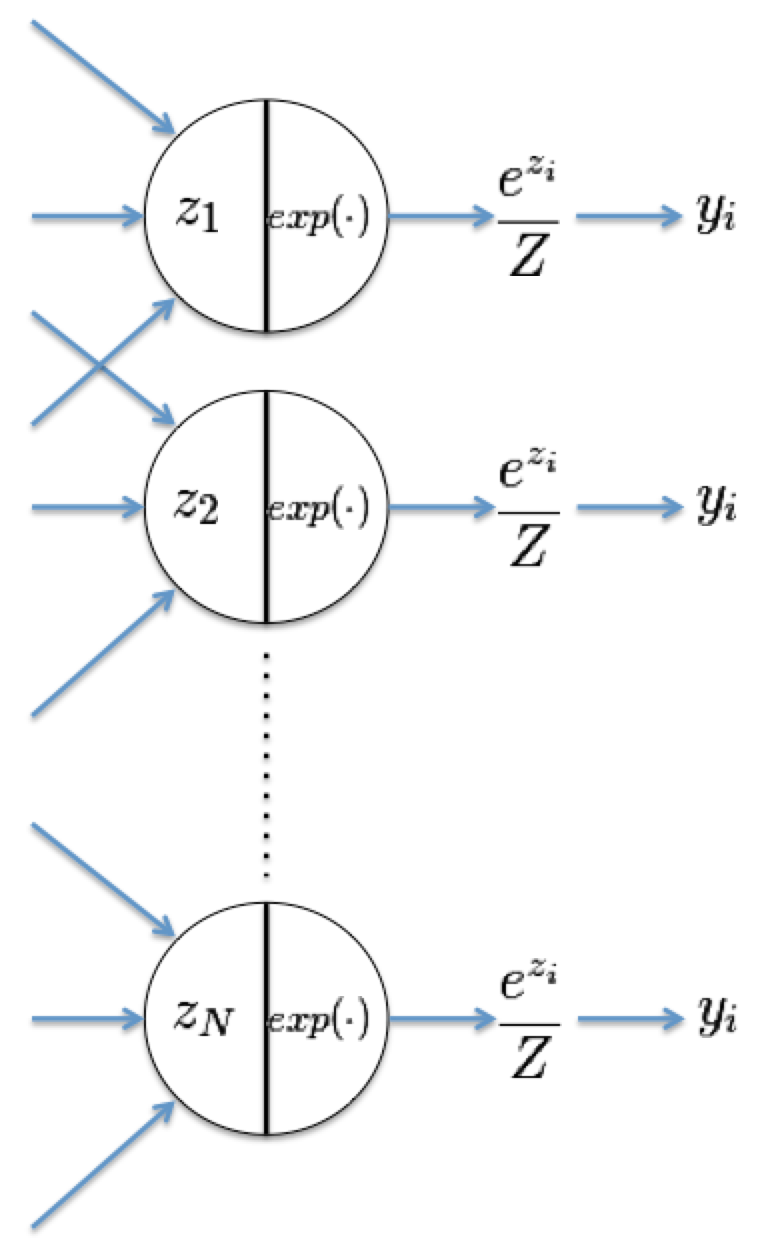
\includegraphics[width=1\textwidth]{images/softmax_layer.png}
    \column{0.6\textwidth}
	\begin{itemize}
		\item $z^{(n)}_j = \sum^{N_{n-1}}_{i=0} w^{(n)}_{ij}x^{(n)}_i$
		\item $y_j = \textsc{softmax}(z_j) = \dfrac{z_j}{Z} = \dfrac{z_j}{\sum_k z_k}$
		\item $E(\vec y, \vec t) = -\sum_{j = 1}^{N_{n - 1}} t_j \cdot \log y_j$
		\item $\dfrac{\partial y^{(n)}_j}{\partial z^{(n)}_j} = $ \textit{???}
	\end{itemize}	    
\end{columns}

\end{frame}


\begin{frame}{Дифференцирование softmax функции}

\begin{eqnarray*}
\dfrac{\partial y^{(n)}_j}{\partial z^{(n)}_j} &=& \frac{\partial}{\partial z_j} \frac{e^{z_j}}{Z} \\
&=& \frac{1}{Z^2} \cdot \left( \frac{\partial e^{z_j}}{\partial z_j}\cdot Z - e^{z_j}\cdot \frac{\partial Z}{\partial z_j}\right) \\
&=& \frac{1}{Z^2} \cdot \left( e^{z_j} Z - e^{z_j}\frac{\partial e^{z_j}}{\partial z_j}\right) \\
&=& \frac{e^{z_j}Z - \left( e^{z_j} \right)^2}{Z^2} = \frac{e^{z_j}}{Z} - \left( \frac{e^{z_j}}{Z} \right)^2 \\
&=& y_j - y_j^2 \\
&=& y_j\cdot (1 - y_j)
\end{eqnarray*}

\end{frame}


\begin{frame}{Вспомним backprop}


\begin{itemize}
	\item $\dfrac{\partial E}{\partial w^{(n)}_{ij}} = \dfrac{\partial E}{\partial z^{(n)}_j} \dfrac{\partial z^{(n)}_j}{\partial w^{(n)}_{ij}}$
	\item $\dfrac{\partial z^{(n)}_j}{\partial w^{(n)}_{ij}} = \sum_i \dfrac{\partial w^{(n)}_{ij} x_i^{(n - 1)}}{\partial w^{(n)}_{ij}} = x_i^{(n - 1)}$
\end{itemize}
В итоге получим: 
\begin{equation}\label{eq:de_dw}
	\dfrac{\partial E}{\partial w^{(n)}_{ij}} = x_i^{(n - 1)} \dfrac{\partial E}{\partial z^{(n)}_j}
\end{equation}
Продолжим с этого момента, с учетом того, что функцией стоимости является перекрестная энтропия (опустим индекс слоя для наглядности):
\begin{itemize}
	\item $E(\vec y\left(\vec z\right), \vec t) = -\sum_{j = 1}^{N_{n - 1}} t_j \cdot \log y_j (z_j)$
	\item $\dfrac{\partial E}{\partial z_j} = $ \textit{???}
\end{itemize}

\end{frame}


\begin{frame}{Дифференцирование перекрестной энтропии, \#1}

Раньше было так (для выходного слоя):
\begin{equation*}
	\dfrac{\partial E}{\partial z_j} = \dfrac{\partial E}{\partial y_j} \dfrac{\partial y_j}{\partial z_j}
\end{equation*}

Теперь стало так:
\begin{eqnarray*}
\dfrac{\partial E}{\partial z_j} &=& \sum_{i = 1}^{N_{n}} \frac{\partial E}{\partial y_i} \cdot \frac{\partial y_i}{\partial z_j}
\end{eqnarray*}

\begin{itemize}
	\item \textit{почему так?}
\end{itemize}

\end{frame}


\begin{frame}{Дифференцирование перекрестной энтропии, \#2}

\begin{itemize}
	\item $\dfrac{\partial E}{\partial z_j} = \sum_{i = 1}^{N_{n}} \dfrac{\partial E}{\partial y_i} \cdot \dfrac{\partial y_i}{\partial z_j}$
	\item $\dfrac{\partial E}{\partial y_i}$ \textit{???}
\end{itemize}

\end{frame}


\begin{frame}{Дифференцирование перекрестной энтропии, \#2}

\begin{itemize}
	\item $\dfrac{\partial E}{\partial z_j} = \sum_{i = 1}^{N_{n}} \dfrac{\partial E}{\partial y_i} \cdot \dfrac{\partial y_i}{\partial z_j}$
\end{itemize}

\begin{eqnarray*}
\dfrac{\partial E}{\partial y_i} &=& -\frac{\partial}{\partial y_i} \left( \sum_k^{N_n} t_k\cdot \log y_k \right) \\
&=& -\frac{\partial}{\partial y_i} \left( t_i\cdot \log y_i \right) \\
&=& -\frac{t_i}{y_i}
\end{eqnarray*}

\end{frame}


\begin{frame}{Дифференцирование перекрестной энтропии, \#3}

\begin{itemize}
	\item $\dfrac{\partial E}{\partial z_j} = \sum_{i = 1}^{N_{n}} \dfrac{\partial E}{\partial y_i} \cdot \dfrac{\partial y_i}{\partial z_j}$
	\item $\dfrac{\partial E}{\partial y_i} = -\dfrac{t_i}{y_i}$
	\item $\dfrac{\partial y_i}{\partial z_j}$ \textit{???}
\end{itemize}

\end{frame}


\begin{frame}{Дифференцирование перекрестной энтропии, \#4}

\begin{itemize}
	\item $\dfrac{\partial E}{\partial z_j} = \sum_{i = 1}^{N_{n}} \dfrac{\partial E}{\partial y_i} \cdot \dfrac{\partial y_i}{\partial z_j}$
	\item $\dfrac{\partial E}{\partial y_i} = -\dfrac{t_i}{y_i}$
\end{itemize}

\begin{equation*}
\dfrac{\partial y_i}{\partial z_j} = \left\{ { y_j\left( 1 - y_j \right), i = j \atop\textit{???}, i \neq j} \right.
\end{equation*}

\end{frame}


\begin{frame}{Дифференцирование перекрестной энтропии, \#5}

\begin{itemize}
	\item $\dfrac{\partial E}{\partial z_j} = \sum_{i = 1}^{N_{n}} \dfrac{\partial E}{\partial y_i} \cdot \dfrac{\partial y_i}{\partial z_j}$
	\item $\dfrac{\partial E}{\partial y_i} = -\dfrac{t_i}{y_i}$
	\item $\dfrac{\partial y_i}{\partial z_j} = \left\{ { y_j\left( 1 - y_j \right), i = j \atop\textit{???}, i \neq j} \right.$
\end{itemize}

\begin{eqnarray*}
\dfrac{\partial y^{(n)}_i}{\partial z^{(n)}_j} &=& \frac{1}{Z^2} \cdot \left( \frac{\partial e^{z_i}}{\partial z_j}\cdot Z - e^{z_i}\cdot \frac{\partial Z}{\partial z_j}\right) \\
&=& \frac{1}{Z^2} \left( 0 - e^{z_i}\cdot e^{z_j} \right) \\
&=& -y_i\cdot y_j
\end{eqnarray*}

\end{frame}


\begin{frame}{Дифференцирование перекрестной энтропии, \#6}

\begin{itemize}
	\item $\dfrac{\partial E}{\partial z_j} = \sum_{i = 1}^{N_{n}} \dfrac{\partial E}{\partial y_i} \cdot \dfrac{\partial y_i}{\partial z_j}$
	\item $\dfrac{\partial E}{\partial y_i} = -\dfrac{t_i}{y_i}$
	\item $\dfrac{\partial y_i}{\partial z_j} = \left\{ { y_j\left( 1 - y_j \right), i = j \atop -y_i y_j, i \neq j} \right.$
	\item $\dfrac{\partial E}{\partial y_i} \cdot \dfrac{\partial y_i}{\partial z_j} = \left\{ { -t_j\left(1 - y_j\right), i = j \atop y_j t_i, i \neq j } \right.$
	\item собираем все вместе
\end{itemize}

\end{frame}


\begin{frame}{Дифференцирование перекрестной энтропии, \#7}

\begin{itemize}
	\item $\dfrac{\partial E}{\partial z_j} = \sum_{i = 1}^{N_{n}} \dfrac{\partial E}{\partial y_i} \cdot \dfrac{\partial y_i}{\partial z_j}$
	\item $\dfrac{\partial E}{\partial y_i} \cdot \dfrac{\partial y_i}{\partial z_j} = \left\{ { -t_j\left(1 - y_j\right), i = j \atop y_j t_i, i \neq j } \right.$
\end{itemize}

\begin{eqnarray*}
\dfrac{\partial E}{\partial z_j} &=& -t_j\left(1 - y_j\right) + \sum_{i = 1, i \neq j}^{N_{n}} y_j t_i \\
&=& -t_j + t_j y_j + y_j \cdot \sum_{i = 1, i \neq j}^{N_{n}} t_i \\
&=& -t_j + y_j \left(t_j + \cdot \sum_{i = 1, i \neq j}^{N_{n}} t_i \right) \\
&=& ???
\end{eqnarray*}

\end{frame}

\begin{frame}{Дифференцирование перекрестной энтропии, \#8}

\begin{itemize}
	\item $\dfrac{\partial E}{\partial z_j} = \sum_{i = 1}^{N_{n}} \dfrac{\partial E}{\partial y_i} \cdot \dfrac{\partial y_i}{\partial z_j}$
	\item $\dfrac{\partial E}{\partial y_i} \cdot \dfrac{\partial y_i}{\partial z_j} = \left\{ { -t_j\left(1 - y_j\right), i = j \atop y_j t_i, i \neq j } \right.$
\end{itemize}

\begin{eqnarray*}
\dfrac{\partial E}{\partial z_j} &=& -t_j\left(1 - y_j\right) + \sum_{i = 1, i \neq j}^{N_{n}} y_j t_i \\
&=& -t_j + t_j y_j + y_j \cdot \sum_{i = 1, i \neq j}^{N_{n}} t_i \\
&=& -t_j + y_j \left(t_j + \cdot \sum_{i = 1, i \neq j}^{N_{n}} t_i \right) \\
&=& y_j - t_j
\end{eqnarray*}

\end{frame}


\begin{frame}{Softmax слой, выводы}
\begin{figure}[h!]
  \centering
  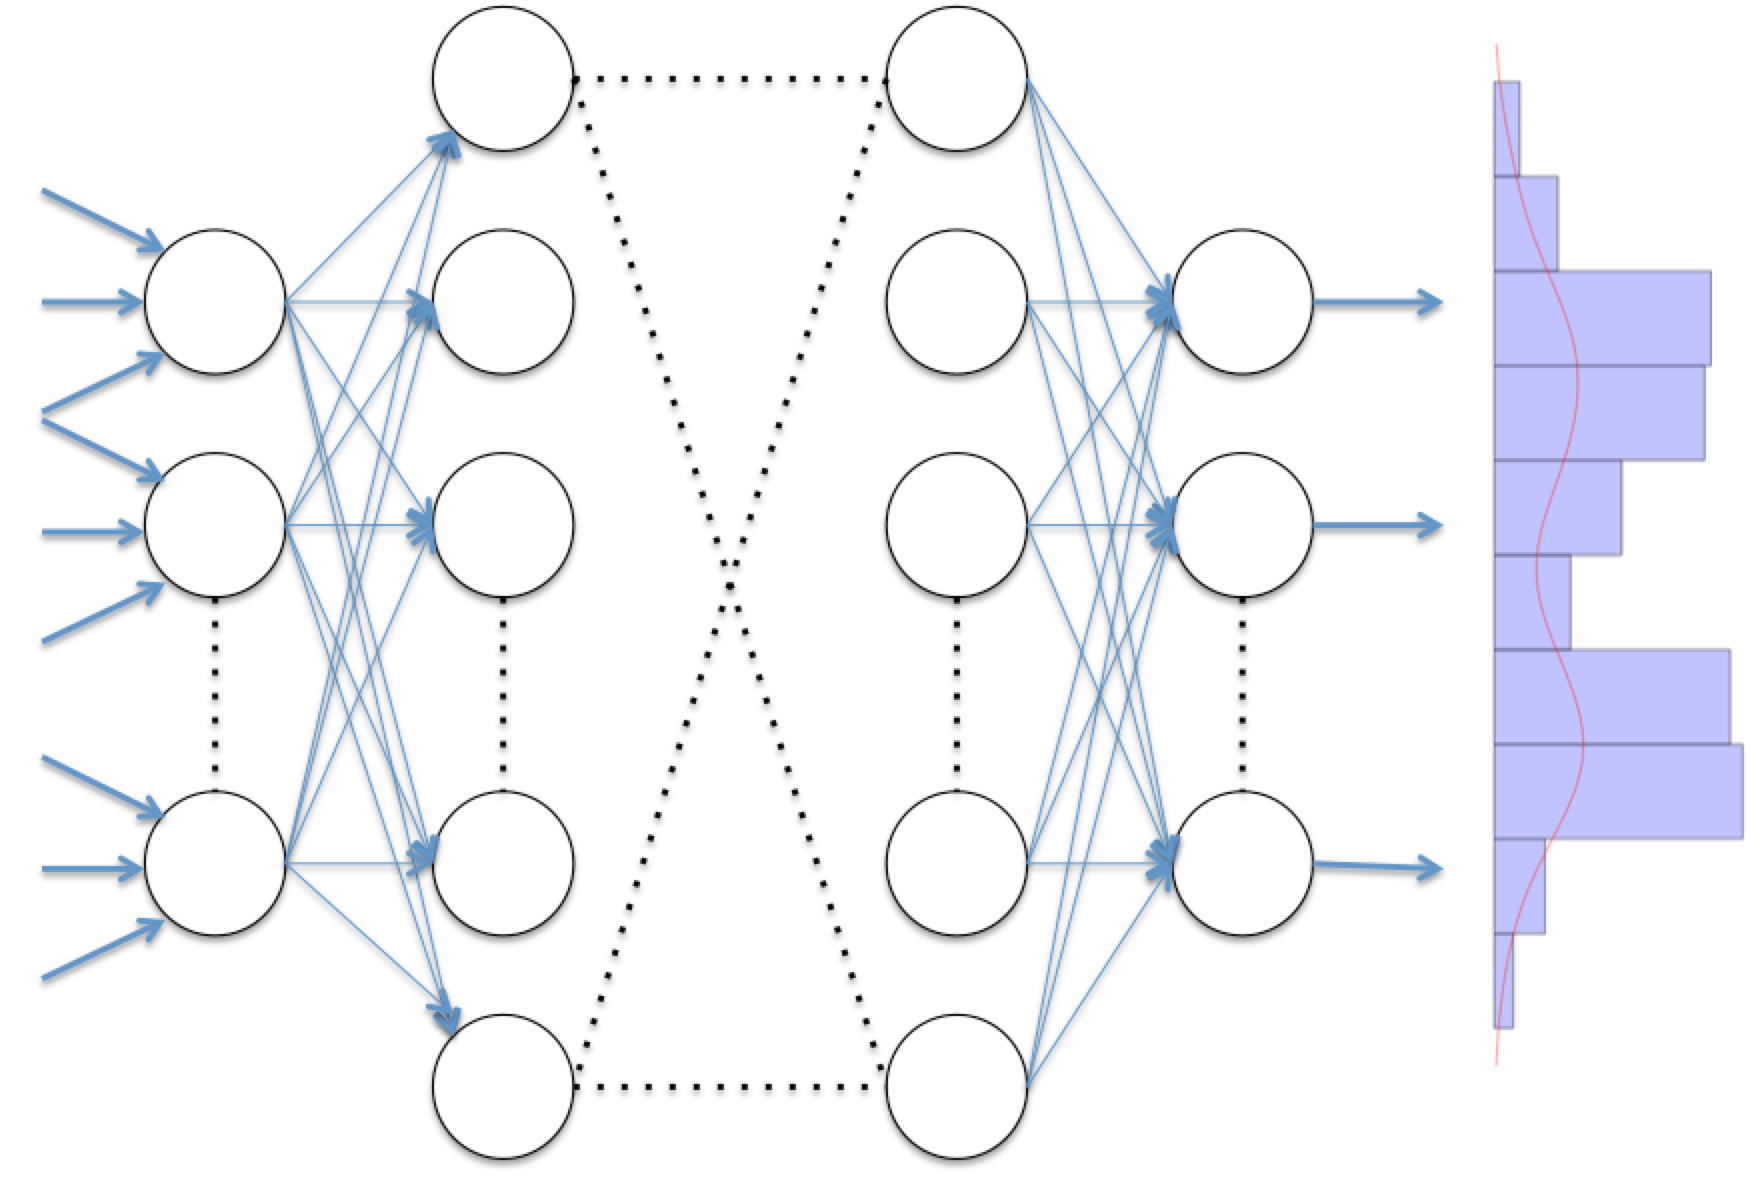
\includegraphics[width=1\textwidth]{images/nn_softmax.png}
\end{figure}
\end{frame}


\section{Обучение без учителя}

\begin{frame}{Обучение без учителя}

\textit{When we’re learning to see, nobody’s telling us what the right answers are — we just look. Every so often, your mother says “that’s a dog”, but that’s very little information. You’d be lucky if you got a few bits of information — even one bit per second — that way. The brain’s visual system has $10^{14}$ neural connections. And you only live for $10^9$ seconds. So it’s no use learning one bit per second. You need more like $10^5$ bits per second. And there’s only one place you can get that much information: from the input itself.}\footnote{Geoffrey Hinton, 1996 (quoted in (Gorder 2006))}

\end{frame}


\begin{frame}{Статистическая механика, \#1}

Представим некоторую физическую систему с множеством степеней свободы, которая может находится в одном из множества состояний с некоторой вероятностью, а каждому такому состоянию состоянию соответствует некоторая энергия всей системы:
\begin{itemize}
	\item $p_i \geq 0$ - вероятность состояния $i$
	\item $\sum_i p_i = 1$
	\item $E_i$ - энергия системы в состоянии $i$
\end{itemize}
Тогда вероятность состояния $i$ будет описываться распределением Больцмана-Гиббса, при условии термодинамического равновесия между системой и окружающей средой:
\begin{equation}
p_i = \frac{1}{Z} \exp \left( -\frac{E_i}{k_B\cdot T} \right)
\end{equation}
где
\begin{itemize}
	\item $T$ - абсолютная температура (К)
	\item $k_B$ - константа Больцмана (Дж/К)
	\item $Z = \sum_i \exp \left( -\frac{E_i}{k_B\cdot T} \right)$ - нормализирующая константа (partition function, Zustadsumme, статсумма)
\end{itemize}

\end{frame}


\begin{frame}{Статистическая механика, \#2}

Два важных вывода:
\begin{enumerate}
	\item состояния с низкой энергией имеют больше шансов возникнуть чем состояния с высокой энергией;
	\item при понижении температуры, чаще всего будут возникать состояния из небольшого подмножества состояний с низкой энергией.
\end{enumerate}

\end{frame}


\begin{frame}{Нейросеть Хопфилда}

\begin{columns}
    \column{0.4\textwidth}
    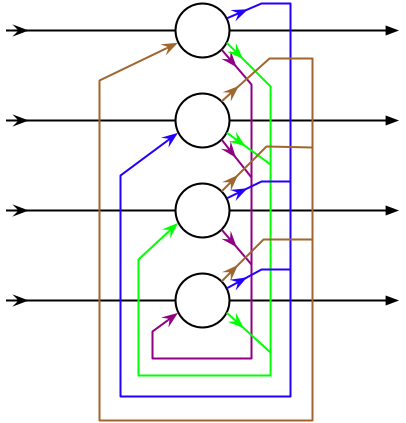
\includegraphics[width=1\textwidth]{images/Hopfield-net.png}
    \column{0.6\textwidth}
	\begin{itemize}
		\item обратная связь
		\item пороговая функция активации
	\end{itemize}	    
	Такая сеть (рекуррентная нейронная сеть) может находится как в стабильном состоянии, осциллировать, или даже проявлять признаки детерминированного хаоса. \\
	Хопфилд показал, что при симметричной матрице весов, существует такая функция энергии бинарных состояний системы, что при симуляции система эволюционирует в одно из низко-энергетических состояний.
\end{columns}

\end{frame}


\begin{frame}{Нейросеть Хопфилда, энергия системы, \#1}

\begin{equation}
E = -\sum_i s_i b_i - \sum_{i < j} s_i s_j w_{ij}
\end{equation}
\begin{itemize}
	\item $s_i$ - состояние нейрона $i$
	\item $b_i$ - смещение нейрона $i$
	\item $w_{ij}$ - вес между нейроном $i$ и $j$
\end{itemize}

\begin{figure}[h!]
  \centering
  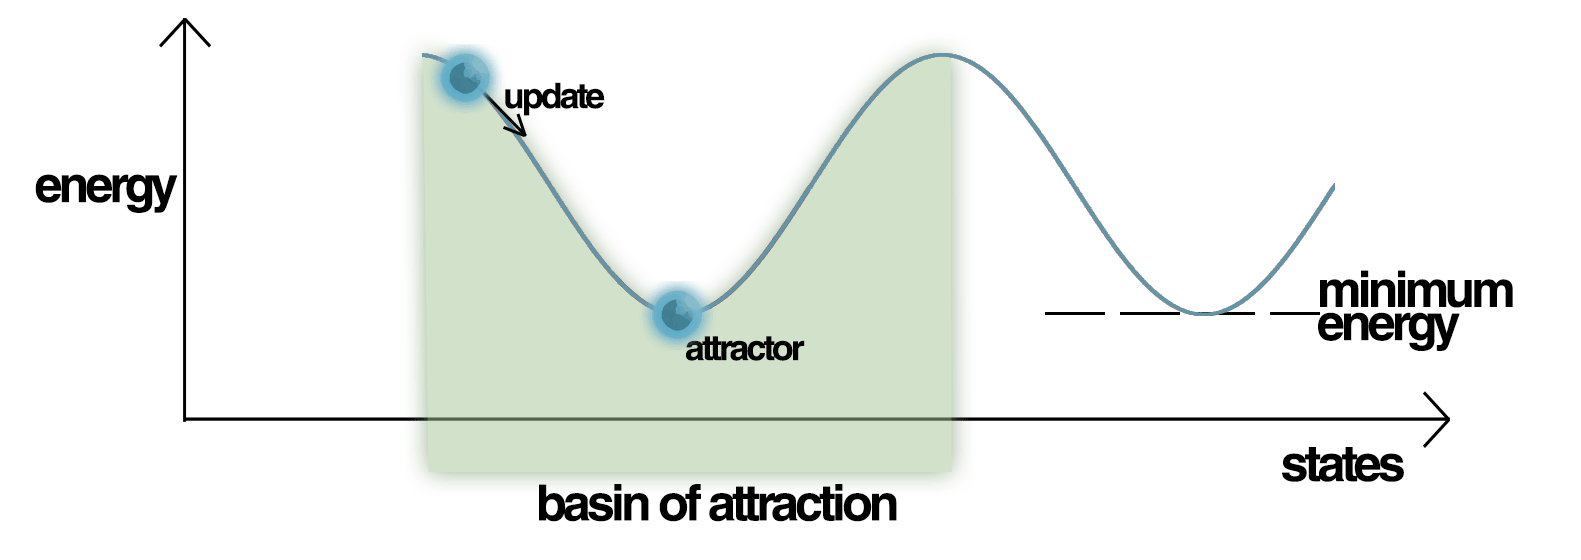
\includegraphics[width=1\textwidth]{images/Energy_landscape.png}
  \caption{Поверхность описываемая энергией сети Хопфилда}
\end{figure}

\end{frame}

\begin{frame}{Нейросеть Хопфилда, энергия системы, \#2}

\begin{figure}[h!]
  \centering
  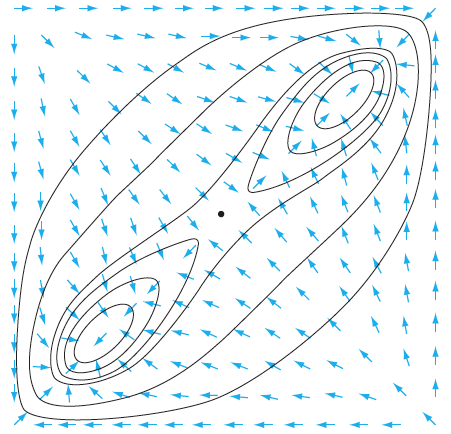
\includegraphics[width=0.6\textwidth]{images/Enegry_countourmap.png}
  \caption{Поверхность описываемая энергией сети Хопфилда, два стабильных состояния\footnote{Neural Networks and Learning Machines (3rd Edition), Simon O. Haykin}}
\end{figure}

\end{frame}


\begin{frame}{Нейросеть Хопфилда, как ассоциативная память}

\begin{figure}[h!]
  \centering
  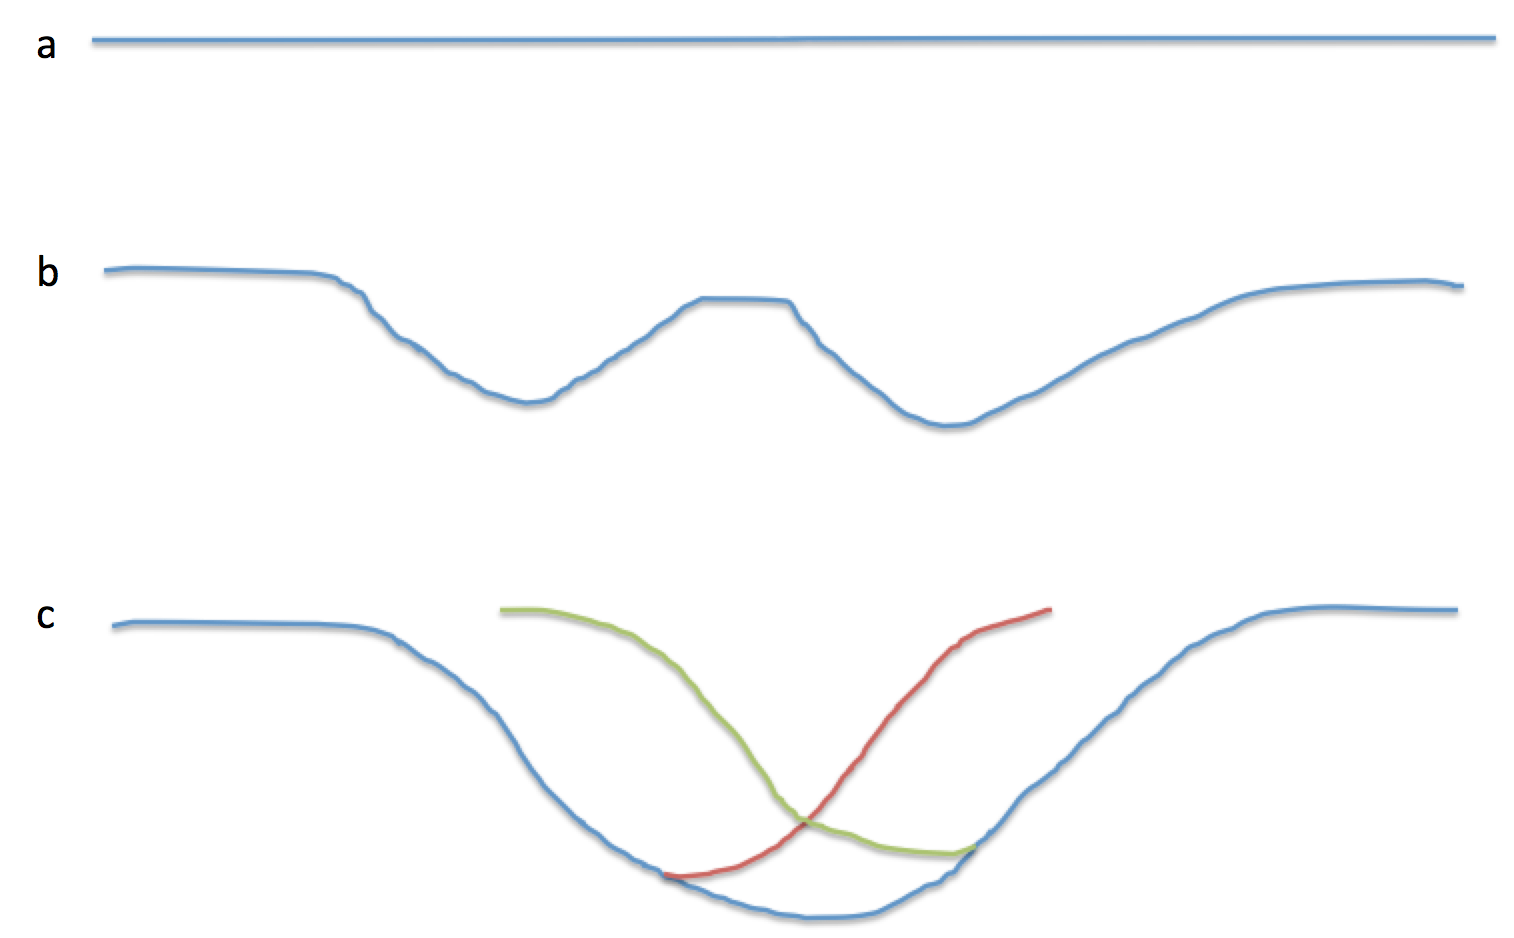
\includegraphics[width=0.6\textwidth]{images/hop_fail.png}
\end{figure}

\begin{itemize}
	\item a - нет образов в памяти
	\item b - два образа далеко друг от друга
	\item c - два образа накладываются друг на друга
\end{itemize}

Вместимость $0.15\cdot N$ на $N$ нейронов.

\end{frame}


\begin{frame}{Нейросеть Хопфилда, алгоритм обучения}

Обучение сети Хопфилда происходит в один прогон по множеству данных по следующему правилу:
\begin{equation}
\Delta w_{ij} = \frac{1}{n} \sum_{i=1}^{n} s_i s_j, \forall k: s_k \in \left\{-1, 1\right\}
\end{equation}

Это в точности первое правило Хебба:
\begin{itemize}
	\item \textit{если два нейрона по разные стороны от синапсов активируются синхронно, то "вес" синапса слегка возрастает}
\end{itemize}

\end{frame}


\begin{frame}{Машина Больцмана - стохастический генеративный вариант сети Хопфилда}

\begin{figure}[h!]
  \centering
  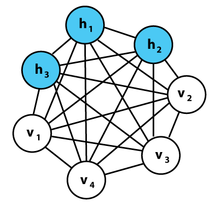
\includegraphics[width=0.4\textwidth]{images/bm.png}
\end{figure}
\begin{itemize}
	\item энергия не изменилась: $E = -\sum_i s_i b_i - \sum_{i < j} s_i s_j w_{ij}$
	\item симметричная матрица весов $w_{ij} = w_{ji}$, но нет обратных связей: $w_{ii} = 0$
	\item появились скрытые состояния (система ищет такую конфигурацию скрытых состояний которая лучшим образом описывает видимые состояния)
	\item $\forall i: s_i \in \left\{0, 1\right\}$
	\item стохастический нейрон
\end{itemize}

\end{frame}


\begin{frame}{Стохастический нейрон}

\begin{figure}[h!]
  \centering
  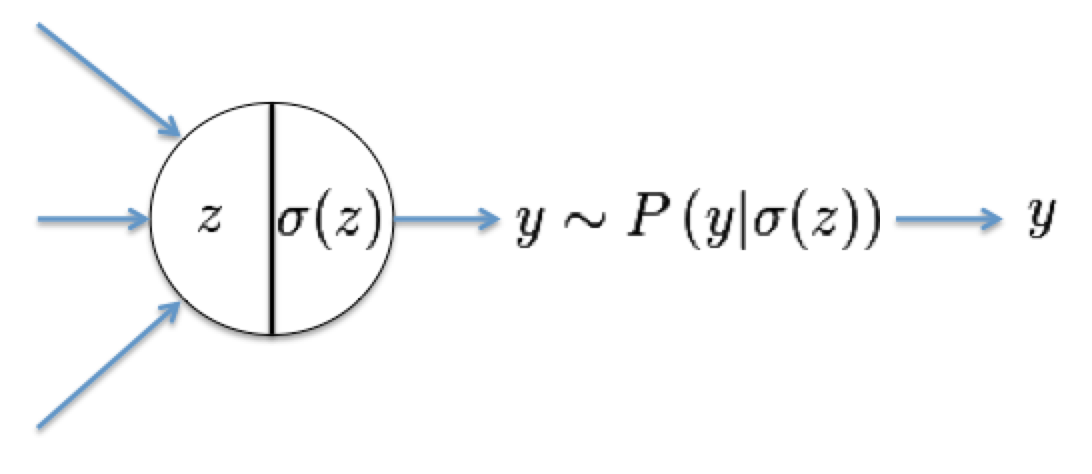
\includegraphics[width=0.7\textwidth]{images/stocastic_neuron.png}
\end{figure}

\end{frame}


\begin{frame}{Имитация отжига, идея, \#1}

\begin{figure}[h!]
  \centering
  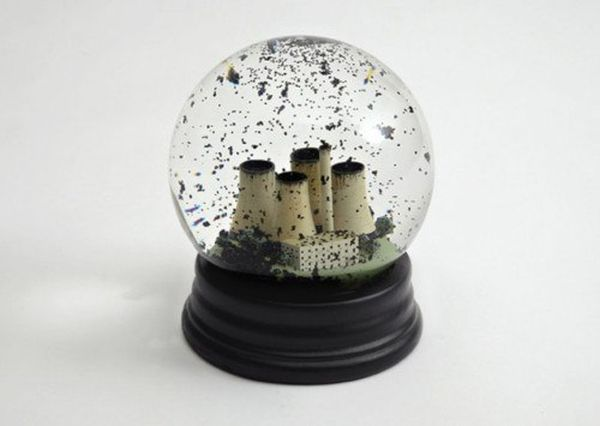
\includegraphics[width=1\textwidth]{images/snowball.jpeg}
\end{figure}

\end{frame}


\begin{frame}{Имитация отжига, идея, \#2}

\begin{figure}[h!]
  \centering
  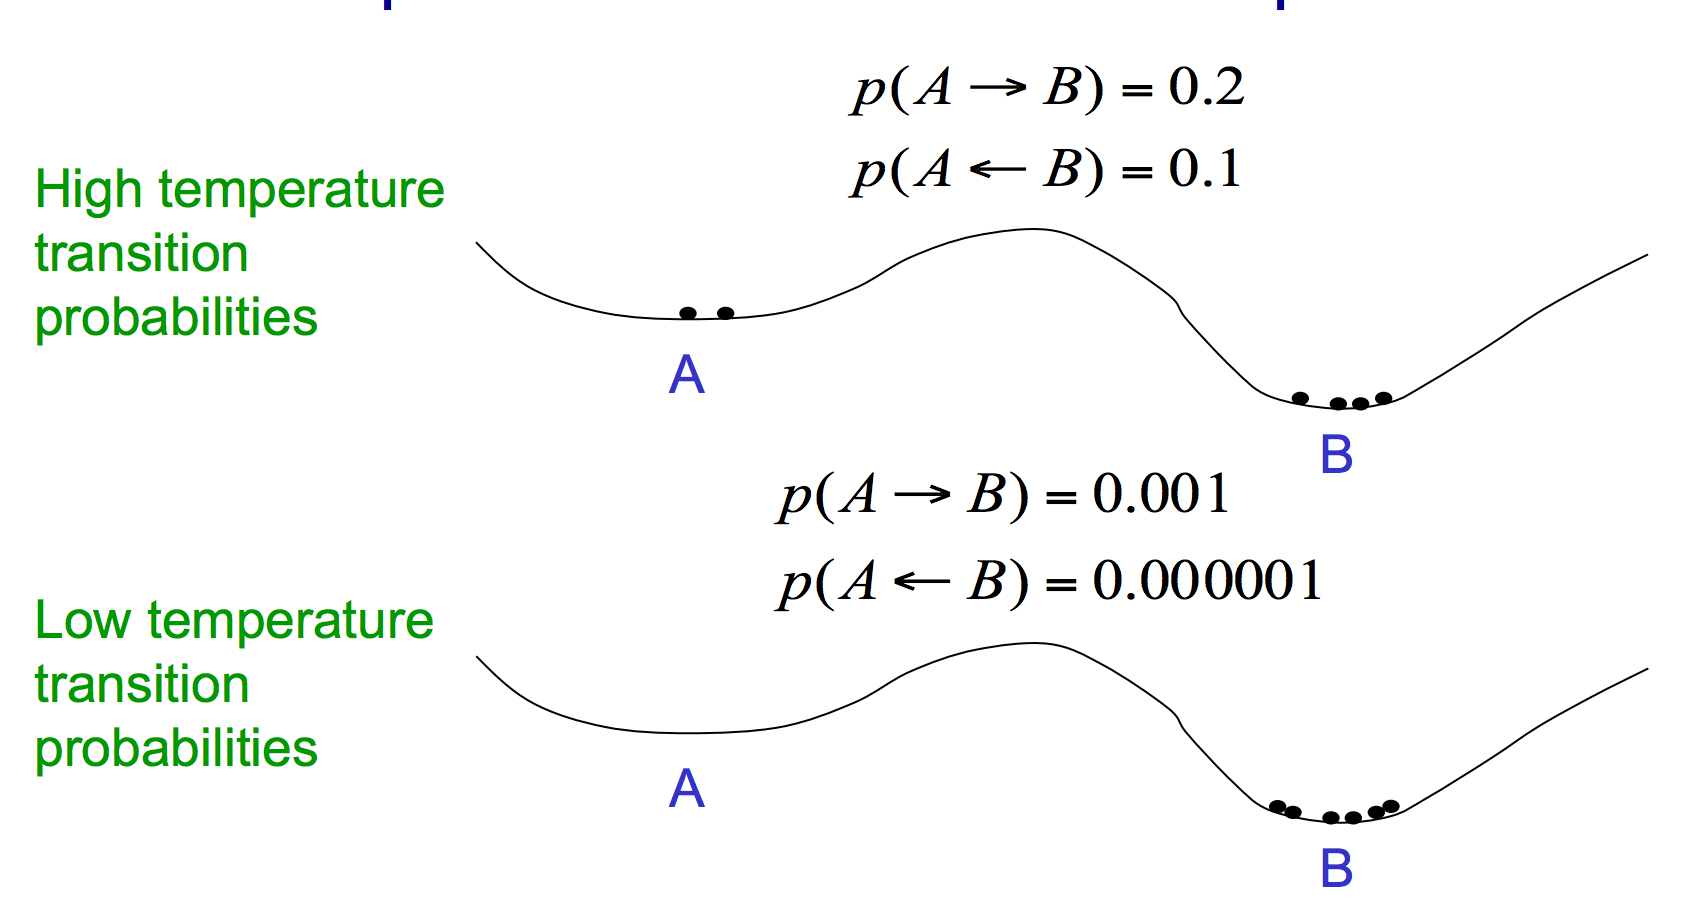
\includegraphics[width=1\textwidth]{images/sim_an.png}
  \caption{Влияние температуры на вероятности переходов\footnote{https://class.coursera.org/neuralnets-2012-001/lecture}}
\end{figure}

\begin{itemize}
	\item SimulatedAnnealing.gif
\end{itemize}

\end{frame}


\begin{frame}{Имитация отжига}

\begin{itemize}
	\item $\Delta E_i = b_i +\sum_j w_{ij}s_j$
	\item $p_i = \frac{1}{Z} \exp \left( -\frac{E_i}{k_B\cdot T} \right)$
\end{itemize}

\begin{eqnarray*}
\frac{p_{i=1}}{p_{i=0}} &=& \exp\left( -\frac{E_{i=0} - E_{i=1}}{k_B T} \right) = \exp\left( \frac{\Delta E_i}{k_B T} \right) \Rightarrow\\
\frac{\Delta E_i}{T} &=& \ln(p_{i = 1}) - \ln(p_{i = 0}) = \ln(p_{i = 1}) - \ln(1 - p_{i = 1})\\
&=& \ln\left(\frac{p_{i = 1}}{1 - p_{i = 1}}\right) \Rightarrow\\
-\frac{\Delta E_i}{T} &=& \ln\left(\frac{1 - p_{i = 1}}{p_{i = 1}}\right) \\
&=& \ln\left(\frac{1}{p_{i = 1}} - 1\right) \Rightarrow \\
\exp\left(-\frac{\Delta E_i}{T}\right) &=& \frac{1}{p_{i = 1}} - 1 \Rightarrow\\
p_{i=1} &=& \dfrac{1}{1 + \exp\left(-\frac{\Delta E_i}{T}\right)}
\end{eqnarray*}

\end{frame}


\begin{frame}{Машина Больцмана - выводы}

Теоретически такая модель может все (как обычно в нейросетях), но
\begin{itemize}
	\item время требуемое для обучения такой модели экспоненциально зависит от размера машины 
	\item по этой же причине нет возможности вычислить $Z$
	\item так же приходится использовать семплирование Гиббса\footnote{Семплирование по Гиббсу не требуется явно выраженное совместное распределение, а нужны лишь условные вероятности для каждой переменной, входящей в распределение. Алгоритм на каждом шаге берет одну случайную величину и выбирает ее значение при условии фиксированных остальных. Можно показать, что последовательность получаемых значений образуют возвратную цепь Маркова, устойчивое распределение которой является как раз искомым совместным распределением.}, в связи с топологией сети (\textit{почему?})
\end{itemize}
\begin{figure}[h!]
  \centering
  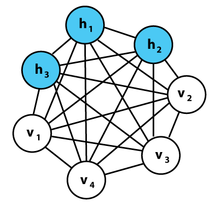
\includegraphics[width=0.3\textwidth]{images/bm.png}
\end{figure}

\end{frame}

\section{Ограниченная машина Больцмана}

\begin{frame}{Ограниченная машина Больцмана}

\begin{itemize}
	\item убираем температуру
	\item вводим \textit{ограничение} на топологию
\end{itemize}

\begin{figure}[h!]
  \centering
  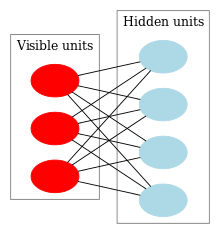
\includegraphics[width=0.5\textwidth]{images/rbm_graph.png}
\end{figure}

\end{frame}


\begin{frame}{Виды RBM}

В зависимости от априрного распределения ассоциированного с видимым и скрытым слоями, различают несколько видов RBM:
\begin{itemize}
	\item Bernoulli-Bernoulli (binary-binary)
	\item Gaussian-Bernoulli
	\item Gaussian-Gaussian
	\item Poisson-Bernoulli
	\item и т.д.
\end{itemize}

Бинарные (Bernoulli-Bernoulli, binary-binary) RBM играют важную роль в глубоком обучении, по аналогии с выводом алгоритма обучения для бинарной ограниченной машины Больцмана, можно вывести аналогичные правила для остальных типов моделей.

\end{frame}


\begin{frame}{RBM, обозначения}

\begin{itemize}
	\item $D = \left\{ \vec x_i \right\}_{i=1\ldots N}$ - множество данных;
	\item $\vec v$, $\vec h$ - значения видимых и скрытых нейронов;
	\item $\vec a, \vec b, W$ - смещения видимых и скрытых нейронов, и матрица весов;
	\item $n, m$ - количество видимых и скрытых нейронов;
	\item $E(\vec v, \vec h) = -\sum_{i=1}^n a_i v_i - \sum_{j=1}^m b_j h_j - \sum_{i=1}^n \sum_{j=1}^m w_{ij} v_i h_j = -\vec v^T \vec a - \vec h^T \vec b - \vec v^T W \vec b$
	\item $p(\vec v, \vec h) = \frac{1}{Z} e^{-E(\vec v, \vec h)}$
	\item $Z = \sum_r^N \sum_t^M e^{-E(\vec v^{(r)}, \vec h^{(t)})}$
	\item $P(\vec v) = \sum_t^M P(\vec v, \vec h^{(t)}) = \frac{1}{Z} \sum_t^M e^{-E(\vec v, \vec h^{(t)})}$
\end{itemize}
\textit{Далее значки вектора $\vec x$ будут опускаться для простоты.}

\end{frame}


\begin{frame}{RBM, функция активации}

Аналогично обычной машине Больцмана, рассмотрим только для скрытого слоя:
\begin{eqnarray*}
P(h_k = 1 | v) &=& \frac{e^{-E_1}}{e^{-E_1} + e^{-E_0}} \\
&=& \frac{1}{1 + e^{E_1 - E_0}} \\
&=& \frac{1}{1 + e^{-b_k - \sum_i^n v_i w_{ik}}}\\
&=& \sigma\left( b_k + \sum_{i=1}^n v_i w_{ik} \right)
\end{eqnarray*}

\textit{Вопрос:}
\begin{itemize}
	\item $P(h | v) = $ \textit{???}
\end{itemize}

\end{frame}


\begin{frame}{RBM, независимость}

\begin{eqnarray*}
P(h | v) &=& \prod_{j = 1}^m P(h_j | v) \\
P(v | h) &=& \prod_{i = 1}^n P(v_i | h)
\end{eqnarray*}

\end{frame}


\begin{frame}{RBM, целевая функция}

\begin{eqnarray}
E(\vec v, \vec h) &=& -\sum_{i=1}^n a_i v_i - \sum_{j=1}^m b_j h_j - \sum_{i=1}^n \sum_{j=1}^m w_{ij} v_i h_j \\
P(\vec v) &=& \frac{1}{Z} \sum_t^M e^{-E(\vec v, \vec h^{(t)})}
\end{eqnarray}

\begin{itemize}
	\item максимизировать вероятность данных при заданной генеративной модели
	\item \textit{что будем делать?}
\end{itemize}

\end{frame}

\section{Алгоритм contrastive divergence}

\begin{frame}{RBM, дифференцирование P(v), \#1}

\begin{equation*}
E(\vec v, \vec h) = -\sum_{i=1}^n a_i v_i - \sum_{j=1}^m b_j h_j - \sum_{i=1}^n \sum_{j=1}^m w_{ij} v_i h_j
\end{equation*}

\begin{columns}
    \column{0.5\textwidth}
	
	\begin{eqnarray*}
	\frac{\partial E(v, h)}{\partial w_{ij}} &=& ? \\
	\frac{\partial E(v, h)}{\partial a_{i}} &=& ? \\
	\frac{\partial E(v, h)}{\partial b_{j}} &=& ?
	\end{eqnarray*}	  
    
    \column{0.5\textwidth}
	
	\begin{eqnarray*}
	\frac{\partial e^{-E(v, h)}}{\partial w_{ij}} &=& ? \\
	\frac{\partial e^{-E(v, h)}}{\partial a_{i}} &=& ? \\
	\frac{\partial e^{-E(v, h)}}{\partial b_{j}} &=& ?
	\end{eqnarray*}
	
\end{columns}

\end{frame}


\begin{frame}{RBM, дифференцирование P(v), \#2}

\begin{equation*}
E(\vec v, \vec h) = -\sum_{i=1}^n a_i v_i - \sum_{j=1}^m b_j h_j - \sum_{i=1}^n \sum_{j=1}^m w_{ij} v_i h_j
\end{equation*}

\begin{columns}
    \column{0.5\textwidth}
	
	\begin{eqnarray*}
	\frac{\partial E(v, h)}{\partial w_{ij}} &=& -v_i h_j \\
	\frac{\partial E(v, h)}{\partial a_{i}} &=& -v_i \\
	\frac{\partial E(v, h)}{\partial b_{j}} &=& -h_j
	\end{eqnarray*}	  
    
    \column{0.5\textwidth}
	
	\begin{eqnarray*}
	\frac{\partial e^{-E(v, h)}}{\partial w_{ij}} &=& v_i h_j e^{-E(v, h)} \\
	\frac{\partial e^{-E(v, h)}}{\partial a_{i}} &=& v_i e^{-E(v, h)} \\
	\frac{\partial e^{-E(v, h)}}{\partial b_{j}} &=& h_j e^{-E(v, h)}
	\end{eqnarray*}
	
\end{columns}

\end{frame}


\begin{frame}{RBM, дифференцирование P(v), \#3}

\begin{equation*}
Z = \sum_r^N \sum_t^M e^{-E(\vec v^{(r)}, \vec h^{(t)})}
\end{equation*}

\begin{columns}
    \column{0.5\textwidth}

	\begin{eqnarray*}
	\frac{\partial Z}{\partial w_{ij}} &=& ? \\
	\frac{\partial Z}{\partial a_{i}} &=& ? \\
	\frac{\partial Z}{\partial b_{j}} &=& ?
	\end{eqnarray*}
	
	\column{0.5\textwidth}
\end{columns}

\end{frame}


\begin{frame}{RBM, дифференцирование P(v), \#4}

\begin{equation*}
Z = \sum_r^N \sum_t^M e^{-E(\vec v^{(r)}, \vec h^{(t)})}
\end{equation*}

\begin{columns}
    \column{0.5\textwidth}

	\begin{eqnarray*}
	\frac{\partial Z}{\partial w_{ij}} &=& \sum_r^N \sum_t^M v_i^{(r)} h_j^{(t)} e^{-E( v^{(r)},  h^{(t)})} \\
	\frac{\partial Z}{\partial a_{i}} &=& \sum_r^N \sum_t^M v_i^{(r)} e^{-E( v^{(r)},  h^{(t)})} \\
	\frac{\partial Z}{\partial b_{j}} &=& \sum_r^N \sum_t^M h_j^{(t)} e^{-E( v^{(r)},  h^{(t)})}
	\end{eqnarray*}
	
	\column{0.5\textwidth}
\end{columns}

\end{frame}


\begin{frame}{RBM, дифференцирование P(v), \#5}

\begin{eqnarray*}
\frac{\partial P\left( v^{(k)} \right)}{\partial w_{ij}} &=& \frac{1}{Z^2} \left( Z \left( \sum_t^M v_i^{(k)} h_j^{(k)} e^{-E( v^{(r)},  h^{(t)})} \right) \right.\\
& & - \left. \left( \sum_t^M e^{-E( v^{(r)},  h^{(t)})} \right) \left( \sum_r^N \sum_t^M v_i^{(r)} h_j^{(t)} e^{-E( v^{(r)},  h^{(t)})} \right)\right) \\
& & \\
\frac{\partial \ln P\left(v^{(k)}\right)}{\partial w_{ij}} &=& \frac{1}{P\left(v^{(k)}\right)} \frac{\partial P\left(v^{(k)}\right)}{\partial w_{ij}}
\end{eqnarray*}


\end{frame}


\begin{frame}{RBM, дифференцирование P(v), \#6}

\begin{eqnarray*}
\frac{\partial \ln P\left(v^{(k)}\right)}{\partial w_{ij}} &=& v_i^{(k)} \sum_t^M h_j^{(t)} P\left( h^{(t)} | v^{(k)} \right) - \sum_r^N \sum_t^M v_i^{(r)} h_j^{(t)} P\left( h^{(t)}, v^{(k)} \right) \\
&=& ???
\end{eqnarray*}

\end{frame}


\begin{frame}{RBM, дифференцирование P(v), \#7}

\begin{eqnarray*}
\frac{\partial \ln P\left(v^{(k)}\right)}{\partial w_{ij}} &=& \sum_t^M v_i^{(k)} h_j^{(t)} P\left( h^{(t)} | v^{(k)} \right) - \sum_r^N \sum_t^M v_i^{(r)} h_j^{(t)} P\left( h^{(t)}, v^{(k)} \right) \\
&=& M\left[v_i^{(k)} h_j \right]_{\textsc{data}} - M\left[v_i h_j\right]_{\textsc{model}} \\
& & \\
\frac{\partial \ln P\left(v^{(k)}\right)}{\partial a_{i}} &=& v_i^{(k)} - M\left[v_i\right]_{\textsc{model}} \\
& & \\
\frac{\partial \ln P\left(v^{(k)}\right)}{\partial b_{j}} &=& M\left[h_j \right]_{\textsc{data}} - M\left[h_j\right]_{\textsc{model}}
\end{eqnarray*}

\end{frame}


\begin{frame}{RBM, правила обновления}

\begin{eqnarray*}
\Delta w_{ij} &=& \eta\left( M\left[v_i^{(k)} h_j \right]_{\textsc{data}} - M\left[v_i h_j\right]_{\textsc{model}} \right) \\
\Delta a_i &=& \eta\left( v_i^{(k)} - M\left[v_i\right]_{\textsc{model}} \right) \\
\Delta b_j &=& \eta\left( M\left[h_j \right]_{\textsc{data}} - M\left[h_j\right]_{\textsc{model}} \right)
\end{eqnarray*}

\end{frame}

\begin{frame}{Алгоритм Contrastive Divergence}

\begin{itemize}
	\item Цель: собрать достаточную статистику для оценки $M[\cdots]_{\textsc{data}}$ и $M[\cdots]_{\textsc{model}}$
\end{itemize}

\begin{figure}[h!]
  \centering
  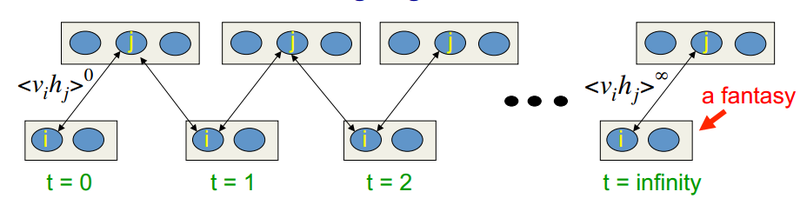
\includegraphics[width=1\textwidth]{images/cd.png}
  \caption{Процесс сбора достаточной статистики\footnote{https://class.coursera.org/neuralnets-2012-001/lecture}}
\end{figure}

\begin{itemize}
	\item $\Delta w_{ij} = \eta \left( M\left[v_i^{(k)} h_j \right]^{(0)} - M\left[v_i h_j\right]^{(\infty)} \right)$
	\item $M\left[\cdots \right]^{(0)}$ - позитивная фаза
	\item $M\left[\cdots\right]^{(\infty)}$ - негативная фаза
\end{itemize}

\end{frame}


\section{Заметки про RBM}

\begin{frame}{Практические советы}

\begin{itemize}
	\item не семплировать видимый слой (семплирование замедляет сходимость, но математически это более корректно);
	\item не семплировать значения скрытого слоя при выводе из восстановленного образа;
	\item CD-$k$, уже при $k=1$ качество не сильно уступает большим значениям, но выигрыш в скорости значительный;
	\item размер минибатча 10-100 экземпляров (\textit{почему?});
	\item кроссвалидаци восстановленных образов;
	\item использование момента сказывается крайне положительно на скорости сходимости;
	\item http://www.cs.toronto.edu/~hinton/absps/guideTR.pdf
\end{itemize}

\end{frame}

\begin{frame}{Визуализация восстановленных образов}

\begin{columns}
    \column{0.2\textwidth}
    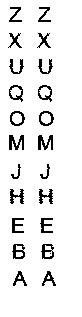
\includegraphics[width=1\textwidth]{images/rec1.png}
    \column{0.8\textwidth}
	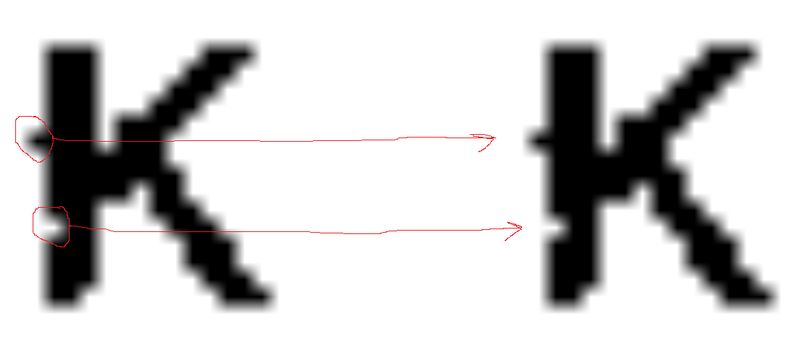
\includegraphics[width=1\textwidth]{images/rec2.png}
\end{columns}

\end{frame}


\begin{frame}{Визуализация признаков, \#1}

\begin{columns}
    \column{0.5\textwidth}
    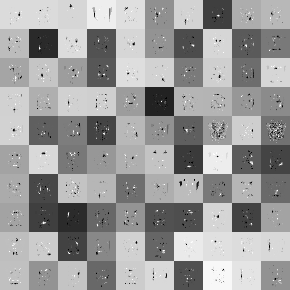
\includegraphics[width=1\textwidth]{images/feats1.png}
    \column{0.5\textwidth}
	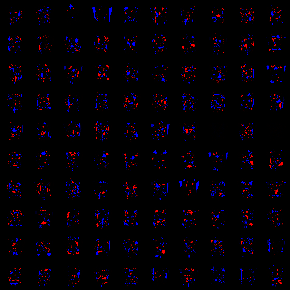
\includegraphics[width=1\textwidth]{images/feats2.png}
\end{columns}

\end{frame}


\begin{frame}{Визуализация признаков, \#2}

\begin{figure}[h!]
  \centering
  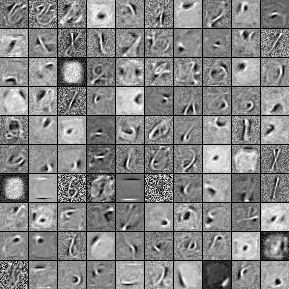
\includegraphics[width=0.5\textwidth]{images/feats3.png}
  \caption{Признаки на множестве рукописных цифр MNIST\footnote{http://deeplearning.net/}}
\end{figure}

\end{frame}


\begin{frame}{Визуализация признаков, \#3}
\begin{figure}[h!]
  \centering
  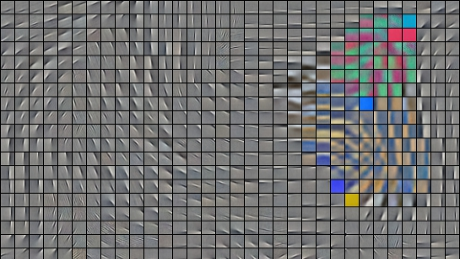
\includegraphics[width=1\textwidth]{images/feats4.png}
\end{figure}
\end{frame}


\begin{frame}{Визуализация признаков, \#4}
\begin{figure}[h!]
  \centering
  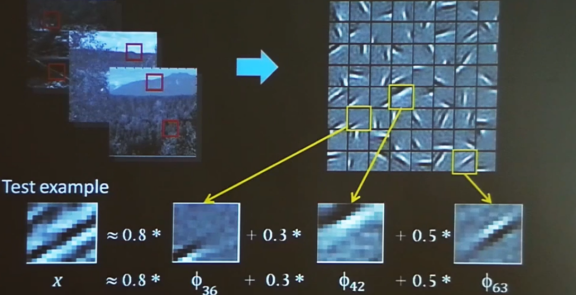
\includegraphics[width=1\textwidth]{images/feats5.png}
  \caption{RBM как базис\footnote{http://cs.stanford.edu/}}
\end{figure}
\end{frame}


\begin{frame}{Регуляризация в RBM, \#1}

\begin{figure}
        \centering
        \begin{subfigure}[b]{0.5\textwidth}
                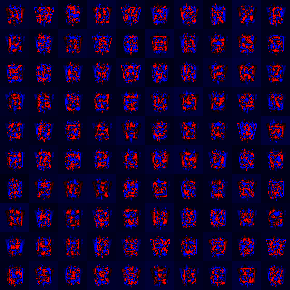
\includegraphics[width=1\textwidth]{images/rbm_colmap_noreg.png}
                \caption{RBM, no reg}                
        \end{subfigure}%        
        \begin{subfigure}[b]{0.5\textwidth}
                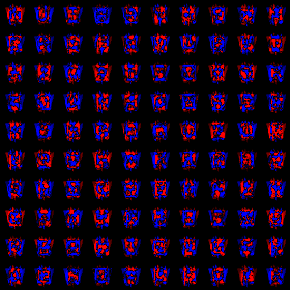
\includegraphics[width=1\textwidth]{images/rbm_colmap_l2.png}
                \caption{RBM, L2 reg}                
        \end{subfigure}       
        \caption{Иллюстрация эффекта регуляризации}
\end{figure}

\end{frame}

\begin{frame}{Регуляризация в RBM, \#2}

\begin{figure}
        \begin{subfigure}[b]{0.5\textwidth}
                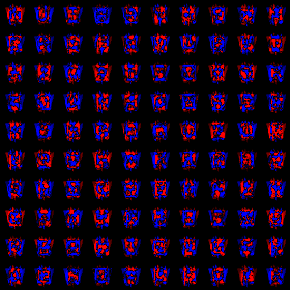
\includegraphics[width=1\textwidth]{images/rbm_colmap_l2.png}
                \caption{RBM, L2 reg}                
        \end{subfigure}%
        \begin{subfigure}[b]{0.5\textwidth}
                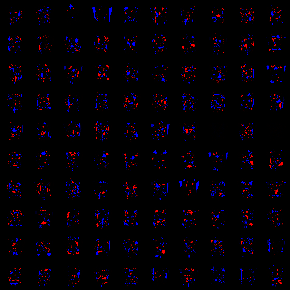
\includegraphics[width=1\textwidth]{images/rbm_colmap_l1.png}
                \caption{RBM, L1 reg}                
        \end{subfigure} 
        \caption{Иллюстрация эффекта регуляризации}
\end{figure}

\end{frame}

\begin{frame}{Критерий остановки}

\begin{figure}[h!]
  \centering
  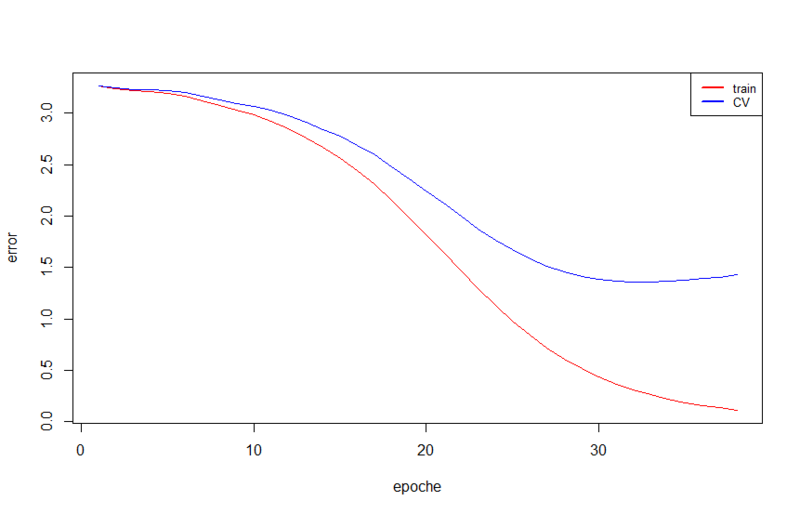
\includegraphics[width=1\textwidth]{images/cv.png}
  \caption{Кроссвалидация}
\end{figure}	
	
\end{frame}


\begin{frame}{Что дальше?}
\begin{figure}[h!]
  \centering
  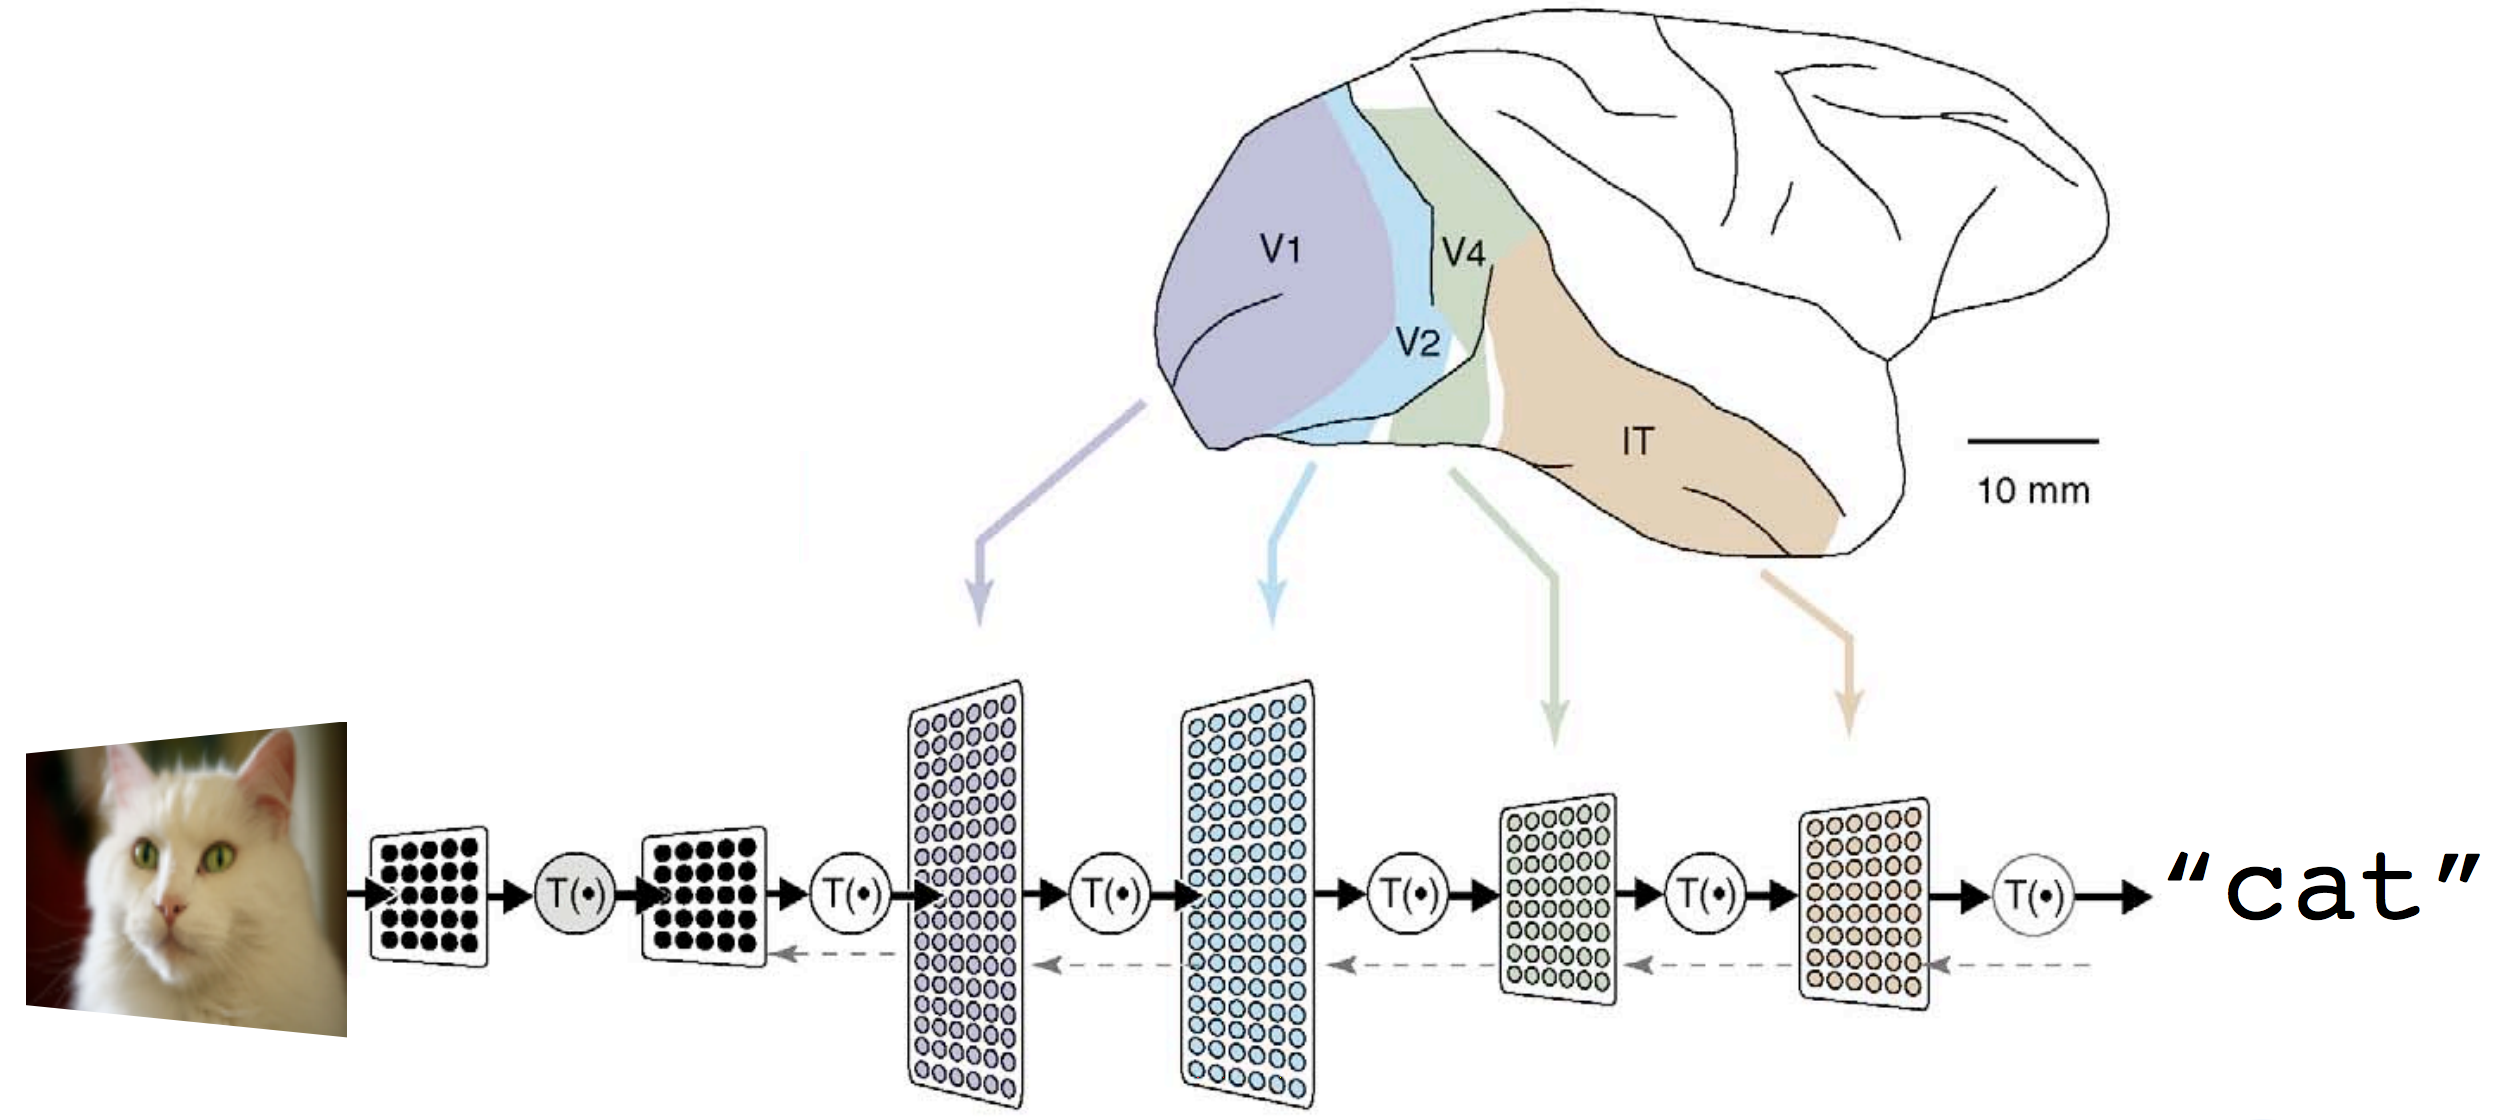
\includegraphics[width=1\textwidth]{images/deepnet1.png}
  \caption{Глубокая нейронная сеть\footnote{Из предентации Scale Deep Learning, Jeff Dean}}
\end{figure}	
\end{frame}



\begin{frame}[plain]
\begin{center}
{\Large Вопросы}
\end{center}
\end{frame}

\end{document}
